\begin{savequote}[6cm]
<< -- Honestly, Spike, don't you know better than to sneak up on ponies?

-- Oh, sorry, but, um, well, isn't that what you're doing?

-- No! I'm doing scientific research. >>
\qauthor{Twilight Sparkle \& Spike}
\end{savequote}

\chapter{Gestion de données pour l'observation}\label{chap:rw:supervision}
\chaptertoc

L'observation est un domaine très actif grâce à l'impact que cela peut avoir dans des situations concrètes (compréhension, diagnostic, autoconfiguration). En dehors des systèmes ad hoc, plusieurs solutions ont été développées pour gérer les données de systèmes. Ce chapitre présente quatre grandes approches que nous avons pu identifier comme intéressantes pour notre problématique.

La section~\ref{sec:rw:supervision:administration} présente les systèmes d'administration, ceux-ci sont déployés depuis plusieurs années pour gérer des parcs de dispositifs à grande échelle et fournissent un grand nombre de données. Afin d'exploiter l'ensemble des données que nous pouvons extraire, nous détaillons la gestion de contexte en section~\ref{sec:rw:supervision:contexte}. Ces systèmes fournissent à une application des informations de contexte pour que celle-ci s'adapte en conséquence.  Puis afin d'extraire et d'analyser les données d'historiques collectées, nous développons l'approche par entrepôts de données en section~\ref{sec:rw:supervision:warehouse}, maintenant largement répandus. Enfin, afin de gérer les données temps réel, les systèmes de gestion de flux de données seront présentés en section~\ref{sec:rw:supervision:datastream}. Ceux-ci permettent de manipuler des flux de données de manière déclarative. Le chapitre~\ref{chap:rw:sgfd} est consacré entièrement à ce thème.

\section{Systèmes d'administrations}\label{sec:rw:supervision:administration}
Les systèmes d'administrations informatiques permettent de gérer des parcs de ressources depuis le début des années 80 avec les premières mises en réseau d'équipements. Le principe étant de surveiller et surtout contrôler un système afin qu'il satisfasse les demandes des utilisateurs et les contraintes du propriétaire~\cite{Sloman:management}. Tant la supervision telle que nous l'entendons dans cette thèse se focalise sur le fait de traiter les données, ici le principe étant d'agir sur les équipements. Toutefois, les systèmes existant sont dotés d'une gestion de données, malheureusement trop ad-hoc la plupart du temps.

Cette section présente les systèmes d'administrations qui se conçoivent encore aujourd'hui pour exploiter des parcs de dispositifs à grande échelle. Ces systèmes sont spécifiés au travers de divers consortiums ou forums tels que le \textit{BroadBand Forum} (BBF) (portés par les opérateurs télécoms), le \textit{Forum Universal Plug'n'Play} (UPnP) (portés par l'électronique grand publique), ou encore \textit{Distributed Management Task Force} (DMTF), l'\textit{Institute of Electrical and Electronics Engineers} (IEEE) et l'\textit{Internet Engineering Task Force} (IETF), organisations ouvertes où participent entreprises, laboratoires et indépendants. Ces ententes permettent la spécification des standards autant au niveau des protocoles de communications que sur les modèles de données manipulés.

Tout d'abord, cette section présente la structure et la gestion des données issues des ressources. Ensuite, nous présenterons l'ensemble des possibilités de traitement. Et enfin, nous synthétiserons cette présentation grâce à la grille d'analyse.
\subsection{Architecture de gestion des données}
L'architecture de la gestion des données dans les systèmes classiques d'administration est principalement fondé sur des gestionnaires agents~\cite{CCITT:X700} (voir fig.~\ref{fig:rw:supervision:administration}). Cette architecture est celle utilisée de nos jours dans les protocoles d'administrations tels que TR-069~\cite{BBF:tr069}, UPnP Device Management~\cite{UPnP:MD}, mais aussi sur des protocoles plus anciens tels que SNMP~\cite{IETF:SNMP}. Le principe étant que sur les dispositifs devant être administrés est présent un module logiciel. Celui-ci comporte un agent capable de maintenir une petite base de données sous un format particulier représentant les données et état du système. Un gestionnaire est capable par la suite de transmettre les informations de l'agent à un système d'administration global qui agrégera l'ensemble des dispositifs.
\begin{figure}[ht]
    \centering
    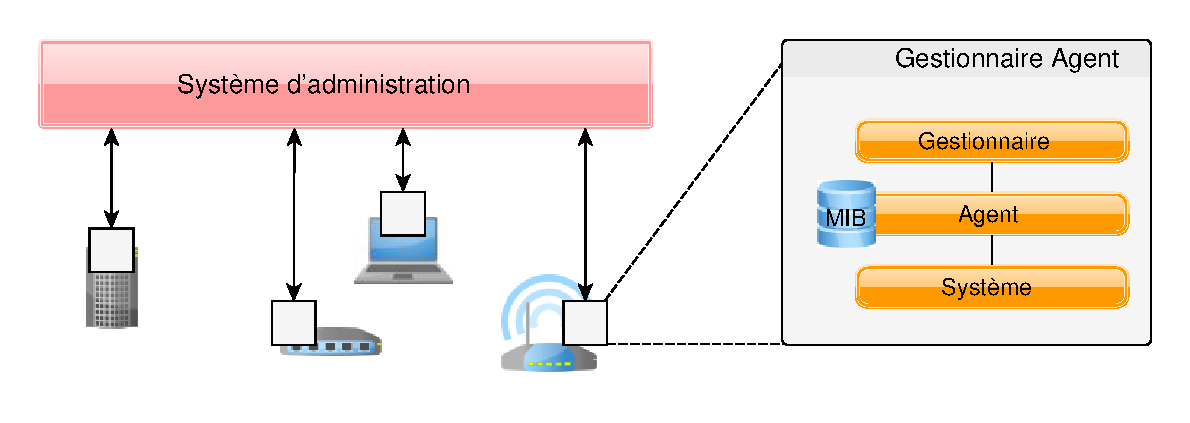
\includegraphics[width=.75\textwidth]{fig/rw-supervision-administration}
    \caption{Architecture d'un système classique d'administration}\label{fig:rw:supervision:administration}
\end{figure}

\subsubsection{Modèles de données}
Il existe plusieurs structures abstraites de données dans le cadre des systèmes d'administrations. La structure la plus répandue reste en l'état la \textbf{structure hiérarchique}. La première apparition d'un tel modèle de donnée remonte à la spécification de SNMP qui prévoit le concept de \textit{Management Information Base} (MIB)~\cite{IETF:MIB}. Une \textit{MIB} est une base d'information où les données sont regroupées sous forme d'arbre. Chaque information possède à l'intérieur de ce arbre un chemin unique (l'\textit{object identifier}) décrit par une suite de chiffres séparés de points. Par exemple, \verb|1.3.6.1.2.1.2.2.1.2| est le chemin décrivant le nom d'une interface réseau sur un dispositif (par exemple \textit{eth0} sur un système Linux). Et le sous-arbre \verb|1.3.6.1.2| (MIB-II~\cite{IETF:MIB-II}) contient toutes les informations concernant les informations réseaux du dispositif.

Par la suite, l'idée des structures hiérarchiques a été reprise pour créer les protocoles d'administrations plus récents comme la structure du modèle des dispositifs de TR-069 (décrit dans le TR-106~\cite{BBF:tr106}) et dans le service de gestion de configuration (CMS) de UPnP-DM~\cite{UPnP:DMCMS}. Dans ces derniers, le modèle de donnée est décrit comme un système de fichier. Les \textit{instances} sont assimilables à des dossiers, et les \textit{feuilles} sont assimilables à des fichiers. Les nœuds ont ainsi un nom et un chemin unique vers la racine \enquote{/}. Tout comme leurs analogues, les \textit{instances} n'ont pas de valeurs associées alors que les \textit{feuilles} contiennent une donnée. Il existe plusieurs types d'\textit{instances} :
\begin{itemize}
    \item \textit{Unique} : Ce nœud peut contenir tout autre nœud. Il représente simplement un chemin intermédiaire un groupe de données.
    \item \textit{Multiple} : Ce nœud peut contenir plusieurs nœuds de type \textit{Instance}. Il permet de représenter une liste de nœuds similaires.
    \item \textit{Instance} : Il représente l'élement de la liste définie par l'instance multiple. Son nom sera toujours un entier pour l'identifier parmi les autres instances. Ces nœuds ont pour vocation à être créés ou supprimés en fonctionnement.
\end{itemize}
\begin{figure}[ht]
    \centering
    \includegraphics[width=.75\textwidth]{fig/rw-supervision-dmtree}
    \caption{Structure hiérarchique du modèle de données d'UPnP-DM}\label{fig:rw:supervision:dmtree}
\end{figure}


Un exemple de modèle de données de ce type de structure est présenté en figure~\ref{fig:rw:supervision:dmtree}. Désormais, une donnée est définie de manière unique, tout comme dans la MIB, grâce à son chemin complet. Dans le vocabulaire du domaine de l'administration, cette donnée est appelé \textit{paramètre}. Le \textit{chemin} d'un paramètre est la concaténation des noms des nœuds qui le sépare de la racine, avec pour séparateur \enquote{/} dans UPnP ou \enquote{.} dans TR-069. Voici quelques exemples de paramètres :
\begin{itemize}
\item \verb|/UPnP/DM/DeviceInfo/PhysicalDevice/HardwareVersion| permet de connaître la version du matériel du dispositif administré. 
\item \verb|/UPnP/DM/Configuration/Network/IPInterface/3/SystemName| est le nom d'une des interfaces réseaux (tout comme \verb|1.3.6.1.2.1.2.2.1.2| dans la MIB). En remplaçant \verb|/3/| par \verb|/5/|, cela concernera une autre interface réseau.
\end{itemize}

L'implémentation de l'agent permettra par la suite de pouvoir créer et remplir cette base d'information.

Toutefois, tous les modèles ne sont pas tous orientés sur la hiérarchie. Il existe notamment l'approche objet adoptée dans les protocoles issues de la DMTF. En effet, dans les protocoles tels que WBEM~\cite{DMTF:WBEM} proposé par le DMTF, la fondation du modèle de données est décrit par un diagramme de classe UML comme présenté en figure~\ref{}.
\begin{figure}[ht]
    \centering
    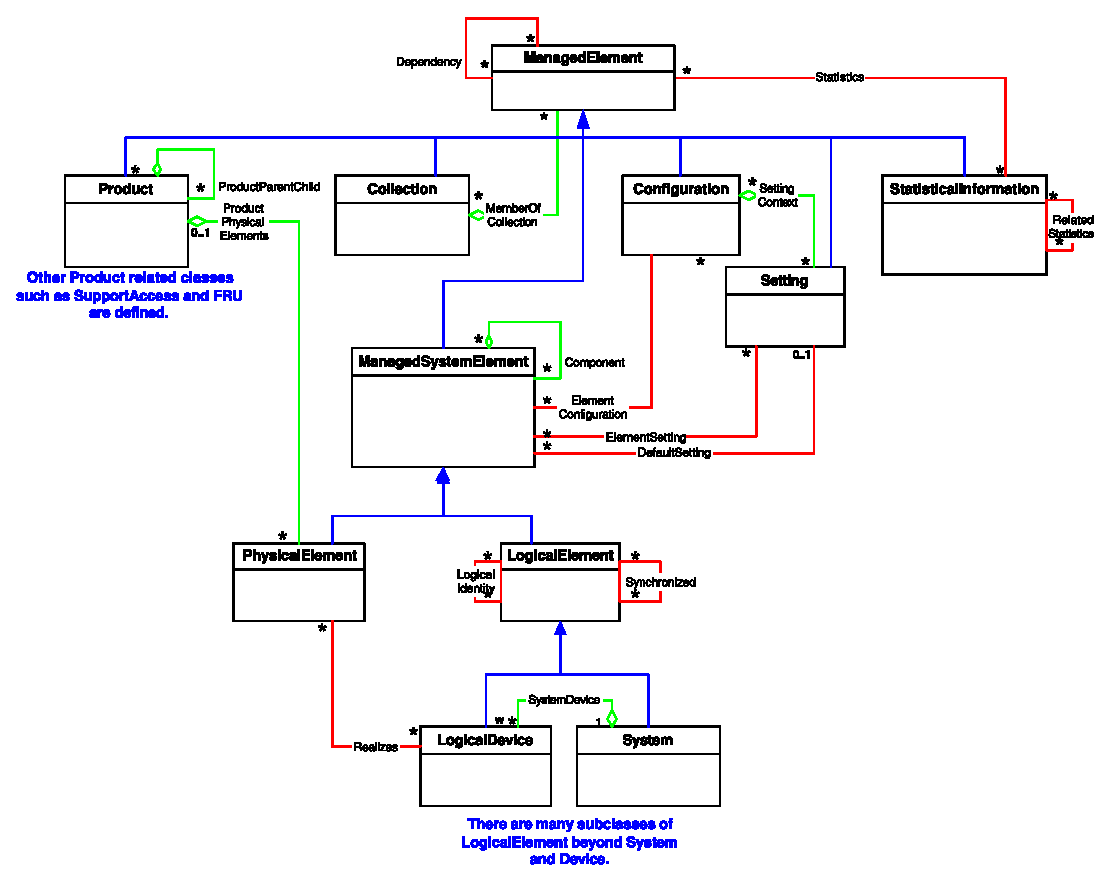
\includegraphics[width=.75\textwidth]{fig/rw-supervision-cimcore}
    \caption{Structure de classe de la partie \textit{Core} de \textit{CIM}}\label{fig:rw:supervision:cimcore}
\end{figure}
\subsubsection{Le gestionnaire global}
Dans l'architecture présentée en figure~\ref{fig:rw:supervision:administration}, 
\subsubsection{Dynamisme des données}
\subsection{Possibles traitements de données}
\subsubsection{L'hétérogénéité par la standardisation}
\subsubsection{Intégration de sources}
\subsubsection{Statistiques}
\subsubsection{Extension du modèle}
\subsection{Synthèse}

\begin{table}[ht]
\criteretabDonnee
    {Principalement structure \textbf{hiérarchique} sous forme de système de fichier. Quelques systèmes d'administration utilisent des modèles objets avec CIM, mais reste difficile à maîtriser.}
    {Une donnée est identifié par son chemin complet. La sémantique est décrite par ce chemin. Pas de contraintes ou inférences exprimées.}
    {Le dynamisme est géré par le mode d'accès. Certains nœuds peuvent être notifiables. D'autres ne sont actualisés que par consultation.}
\criteretabTraitement
    {Instantané et continu sur certaines données. Pas d'hybride possible vu que les procédés sont très séparés.}
    {Standardisation des modèles. Toutes les entités sont structurés dans le même formalisme. Intégration par union des résultats.}
    {Appel de méthodes standardes pour récupérer un sous-arbre du modèle. Code impératif (scripting) pour manipuler les données au niveau du gestionnaire.}
    {Projection simple sur les appels. Certains nœuds particuliers permettent de calculer des statistiques.}
\criteretabAdaptabilite
    {Pas d'adaptation car les dispositifs doivent implémenter des standards.}
    {Pas de perspectives métiers en dehors de la sélection sur les branches du modèle.}
    {Nœuds particuliers pour le calcul. Fonctions métiers intégrées dans le gestionnaire.}
    {Très efficace et utilisé pour gérer des parcs de millions de dispositifs.}
\end{table}
\section{Informatique contextuelle}\label{sec:rw:supervision:contexte}
Au centre des systèmes pervasifs et de l'informatique ubiquitaire, l'informatique contextuelle prend une importance de plus en plus grande. Sa définition a fait l'objet de plusieurs débats au sein de la communauté scientifique. La définition la plus couramment utilisée est : \enquote{L'informatique contextuelle (\textit{context-aware computing} a pour but de permettre aux équipements de fournir de meilleurs services aux utilisateurs par l'utilisation d'informations de contexte}\cite{Han:contextaware}. Ainsi, le point important est de former un ensemble d'information pour que des applications puissent adapter leur fonctionnement. L'instanciation de cette notion de contexte est un processus d'observation de l'environnement dans lequel se trouve l'application.

La section~\ref{sec:rw:supervision:administration} a permis de voir que le système observé peut fournir de grandes quantités de données. Grâce à l'informatique contextuelle, nous souhaitons pouvoir donner de la cohérence à ces données. Ainsi, nous pouvons mieux exploiter leur sémantique et envisager d'effectuer de l'observation de plus haut niveau afin d'établir un diagnostic.

Cette section présente d'abord les définitions et applications de l'informatique contextuelle. Par la suite, nous détaillons la façon dont le contexte est capturé et modélisé. Nous présentons les capacités de traitement sur celui-ci. Enfin, nous analysons différents systèmes pervasifs afin de percevoir la mise en application de cette approche. Nous concluons par une synthèse, détaillant l'adéquation aux critères de notre problématique.

\subsection{Définitions et applications}
La définition de contexte a été elle aussi au cœur de nombreux débats. Après analyse des travaux sur le sujet, le rapport de recherche~\cite{Dey:context} propose la définition suivante : \enquote{\it Un contexte est toute information pouvant être utilisée pour caractériser la situation d'une entité. Cette entité pouvant être une personne, un lieu, ou un objet considéré comme pertinent à l'interaction entre l'utilisateur et le système.}.

Il est important de noter que cette définition est orientée par l'utilisation qui en est faite. Une donnée quelconque peut faire partie d'un contexte si elle est utilisée comme tel. Ainsi, il est nécessaire de voir l'ensemble des utilisations de ce contexte. Celles-ci sont rassemblées dans sept catégories principales~\cite{Soylu:context} : 
\begin{enumerate}
	\item Sélection et recommandations d'informations ou de services.
	\item Présentation et accès à l'information et aux services.
	\item Recherche d'information ou de service.
	\item Adaptation de l'exécution de processus séquentiels.
	\item Modification et reconfiguration d'applications.
	\item Conseil d'actions semi-automatique.
	\item Allocations de ressources.
\end{enumerate}
Les utilisations du contexte sont directement reliées à l'observation, car c'est elle qui permet la construction du contexte.

\subsection{Modélisation et capture du contexte}
Le modèle utilisé pour créer et manipuler le contexte peut être de différentes formes : basé sur des principes d'intelligence artificielle (représentations de connaissances, réseaux bayésiens), le génie logiciel (UML), les bases de données (ER : Entité-Relation) ou d'autres moyens applicatifs (arbres, entrées clefs-valeurs). L'UML et l'ER atteignent rapidement leurs limites d'expressivité. Il devient difficile de manipuler les données dans le cadre de contextes larges et hétérogènes à cause de leur rigidité. Ces modèles permettent d'abstraire une partie du monde ou de la logique pour un usage restreint. Par opposition, la gestion de données issues d'ontologies est moins soumise à cette rigidité.

\subsubsection{Un modèle sous forme de triplet}
Pour représenter l'ensemble des connaissances sur le système, autant en terme de structure que de données, les contextes sont la plupart du temps modélisés comme un réseau sémantique. Le langage communément utilisé pour cela est le RDF (\textit{Resource Description Framework})~\cite{W3C:RDF}, un standard répandu. Son principe est à la fois simple et puissant. Son expression est simple, car toute sa structure est orchestrée par des triplets : Objet, Relation, Valeur. Par exemple, \textit{la télévision} \textbf{est située dans} \textit{le salon}. De même, \textit{le salon} \textbf{est une} \textit{pièce}. L'ensemble des triplets forme un graphe où les objets et valeurs sont des nœuds et les relations sont des liens, d'où l'appellation de \textit{graphe sémantique}~\cite{Minsky:knowledge}. Pour étendre l'expressivité des graphes sémantiques et y apporter la notion de classes, les ontologies se sont développées.

\subsubsection{Les ontologies}
Tel que l'a défini Kalfoglou~\cite{Kalfoglou:ontology}, une ontologie est \textit{une représentation explicite d'une compréhension commune de concepts importants appartenant à un domaine d'intérêt}.
Elle permet de capturer et de représenter une vue simplifiée d'un domaine à travers des concepts prédéfinis. Cela permet un langage commun et une taxonomie des concepts, mais aussi, l'ontologie est capable de représenter leurs liaisons. Ainsi, il est possible de modéliser la sémantique propre des différentes données.

Les ontologies sont toutefois structurées dans un langage qui permet de définir les grandes catégories de relations ou d'objets. Plusieurs langages existent, mais tous définissent les entités suivantes :
\begin{itemize}
    \item[\textbf{Concepts}] Décrivent les classes et sous-classes de toutes les choses du monde.
    \item[\textbf{Instances}] Ce sont les individus correspondant aux concepts.
    \item[\textbf{Relations}] Permet de lier les concepts et instances entre eux. Une des relations principales est la relation \textit{Est-Un} (\textit{Is-A} en anglais) qui lie une instance à un concept.
    \item[\textbf{Types de données}] Types syntaxique d'une donnée : entier, chaîne de caractères, booléen.
    \item[\textbf{Valeurs}] Valeur qu'un concept ou instance peut avoir.
\end{itemize}

Par la suite, les langages permettent différentes manières de lier les concepts entre eux. Cette capacité va permettre de montrer l'expressivité de la structure. Par exemple, une des relations des plus importantes est la relation de hiérarchie. Un \textit{chien} \underline{est une sous-classe d}'\textit{animal}, et \textit{labrador} \underline{est une sous-classe de} \textit{chien}. La \textit{relation de hiérarchie} \underline{est une} \textit{relation transitive}. Ainsi, le langage vérifie naturellement que le \textit{labrador} \underline{est une sous-classe d}'\textit{animal}. 

La logique permettant d'exprimer ces contraintes et inférences structurelles est une logique de description. Suivant la classe de la logique de description sous-jacente, le langage est plus ou moins complexe à traiter par la suite\footnote{Dans certains cas, comme OWL-Full, son expressivité est tellement large qu'il devient indécidable de vérifier si un concept appartient à une classe.}. Par exemple, le langage le plus utilisé reste \textit{OWL Lite}, équivalent à la logique $\mathcal{SHIF}^\mathcal{(D)}$. Cette logique permet lors de la description des concepts l'utilisation des constructeurs suivants : quantification universelle, négation\footnote{Si la négation et la quantification universelle existent, alors le prédicat d'existence est autorisé, car $\not\forall \equiv \exists$}, transitivité de relation, inversion de relation, hiérarchie de relations. De plus, l'usage de propriétés fonctionnelles et de données est possible. En revanche, la restriction d'une collection à un nombre d'éléments donné par exemple n'est pas possible. Son utilisation est répandue, car les inférences sont calculables dans la pratique contrairement à des logiques plus expressives.

Comparées à des structures telles qu'UML, les ontologies jouissent de la flexibilité des réseaux sémantiques. Il est toutefois important de noter que cette puissance et cette liberté rendent sa manipulation délicate. En effet, il est supposé que toutes les sources de connaissances s'appuient sur une ontologie commune. Il est important d'être minutieux dans la manipulation de cette structure pour éviter par exemple des duplications de concepts, voire des conflits de définitions.

\subsubsection{Capture du contexte}
La capture du contexte est la manière de récupérer une information et de la représenter sous la forme choisie lors de la modélisation. Par exemple, un capteur de température peut insérer un ensemble de triplets pour indiquer qu'à 10h25 le lundi 26 avril, il faisait 25.256ºC sur la source T75896. Cet ensemble de triplets dépend de la modélisation des concepts qui forme le contexte. Lors de la capture, les données sont issues du système observé ou par l'extraction de nouvelles connaissances construites à partir d'informations déjà capturées.

La gestion de l'hétérogénéité est rarement mentionnée puisque les sources de données sont censées être conformes au schéma commun. Toutefois, comme présenté dans~\cite{Kaed:these}, il est possible d'aligner les modèles des sources avec un schéma commun. Le formalisme des ontologies permet en effet de décrire les équivalences logiques entre différents concepts ce qui permet l'intégration de données.

\subsection{Capacités de traitement}
Un intérêt des réseaux sémantiques est le pouvoir de raisonnement logique. Le but ici est de pouvoir inférer de nouveaux triplets à partir des connaissances accumulées. Pour cela, il existe plusieurs langages permettant de spécifier ces inférences. Le plus courant est le langage associé à \textit{RDF} : \textit{SPARQL}. Ce langage a la particularité d'être aussi expressif que l'algèbre relationnelle~\cite{Angles:sparql}\footnote{Plus exactement, SparQL est équivalent au \textit{datalog} non récursif avec négation, ce qui est équivalent à l'algèbre relationnelle.}. Ainsi, il est possible de faire des inférences du premier ordre sur ces données.

Ces inférences sont de trois types :
\begin{itemize}
 \item[\textbf{Association directe}] Une information bas-niveau est associée à une information haut-niveau 
 \item[\textbf{Fusion de contexte}] Un ensemble de données infère un nouvel état 
 \item[\textbf{Fission de contexte}] Une donnée infère un ensemble d'informations
\end{itemize}

Dans l'informatique contextuelle, il est important de distinguer plusieurs espaces de données~\cite{Padovitz:agent} :
\begin{itemize}
 \item[\textbf{L'espace de valeur}] Par exemple, pour une personne, son age est compris entre 0 et 125.
 \item[\textbf{L'espace applicatif}] L'ensemble des données atomiques qui représentent le contexte dit de bas-niveau.
 \item[\textbf{L'espace de situation}] Reflète les situations pouvant être extraites de l'espace applicatif.
\end{itemize}

À un instant donné, il est possible de définir un \textbf{état de contexte} en tant que collection d'attributs de l'espace de contexte. Cet état peut par la suite inférer un ensemble de situations. La figure~\ref{rw-supervision-contextreasoning} résume la structure abstraite du raisonnement sur les contextes.

\begin{figure}[ht]
    \centering
    \includegraphics[width=.50\textwidth]{rw-supervision-contextreasoning}
    \caption{Structure abstraite du raisonnement sur contexte. À un élément du contexte $c_i$ est associée une valeur du domaine $V_i$. À partir de l'espace du contexte $C$, on effectue des associations, des fissions ou fusions pour inférer l'espace des situations $S$.}\label{rw-supervision-contextreasoning}
\end{figure}

\subsubsection{La qualité de contexte}
La qualité du contexte~\cite{Buchholz:quality} est définie comme toute information permettant de décrire la qualité des informations contenues dans le contexte. Le point crucial est que cette qualité n'est pas liée à un quelconque processus ou matériel. Elle peut se décliner en plusieurs \textit{paramètres} : précision, fiabilité, confiance, fraicheur,\dots{}

La qualité des données a des impacts lors du diagnostic. Supposons que nous constatons un problème de pixélisation TV. Cette situation a été inférée par la valeur actuelle d'une métrique indiquant le nombre d'images non décodées. Premièrement, si la source de donnée remontant la métrique n'est pas assez fiable, nous pouvons mettre en doute les relevés. De plus, il est possible que l'information ne reflète pas l'état actuel. Ainsi, la situation indiquant un problème est vraie à la qualité des sources près.

De plus, si nous souhaitons effectuer un diagnostic, nous pouvons indiquer au système que ce type de panne est dû à un problème de lenteur de réseau interne. Toutefois, ce peut être dû à des dysfonctionnements plus rares, comme une panne matérielle. Ainsi, certaines recherches permettent d'introduire une part de probabilités dans les raisonnements pourtant déterministes a priori~\cite{Padovitz:agent}.

Dans cette thèse, nous ne détaillons pas le concept de qualité des données. Néanmoins, nous pouvons voir que cela peut avoir des impacts majeurs. L'utilisation de ces travaux serait intéressant pour des améliorations futures.

\subsection{Analyse de systèmes d'observation à base de contextes existants}
Dans cette partie, nous analysons des systèmes pervasifs à base de contexte existant. Ceux-ci sont en général très utilisés dans le réseau domestique qui est l'environnement de développement le plus courant dans le domaine de l'informatique ubiquitaire. Cette étude nous permet de voir comment est mise en pratique l'approche présentée jusqu'ici.

\subsubsection{De la représentation du système}
\textit{DogOnt}~\cite{Bonino:dogont}, a pour objectif de pouvoir modéliser les objets des environnements domotiques intelligents. Ainsi, en plongeant l'ensemble des équipements au niveau conceptuel des ontologies, il est possible de résoudre les problèmes d'interopérabilité et d'hétérogénéité des données. \textit{DogOnt} est capable de répondre à des requêtes telles que : la position de l'équipement, ses capacités, ses moyens de communication, comment l'environnement est composé (notamment architecturalement parlant, ce qui permet de représenter la maison).

Ainsi, une représentation de haut niveau permet de poser tous les concepts afin de représenter le réseau domestique au sens large. D'une manière plus concrète, un équipement est représenté en tant que \enquote{\it Controllable} (et ses sous-classes). Cette ontologie est représentée dans la figure~\ref{fig:rw:supervision:dogont}.

\begin{figure}[ht]
    \centering
    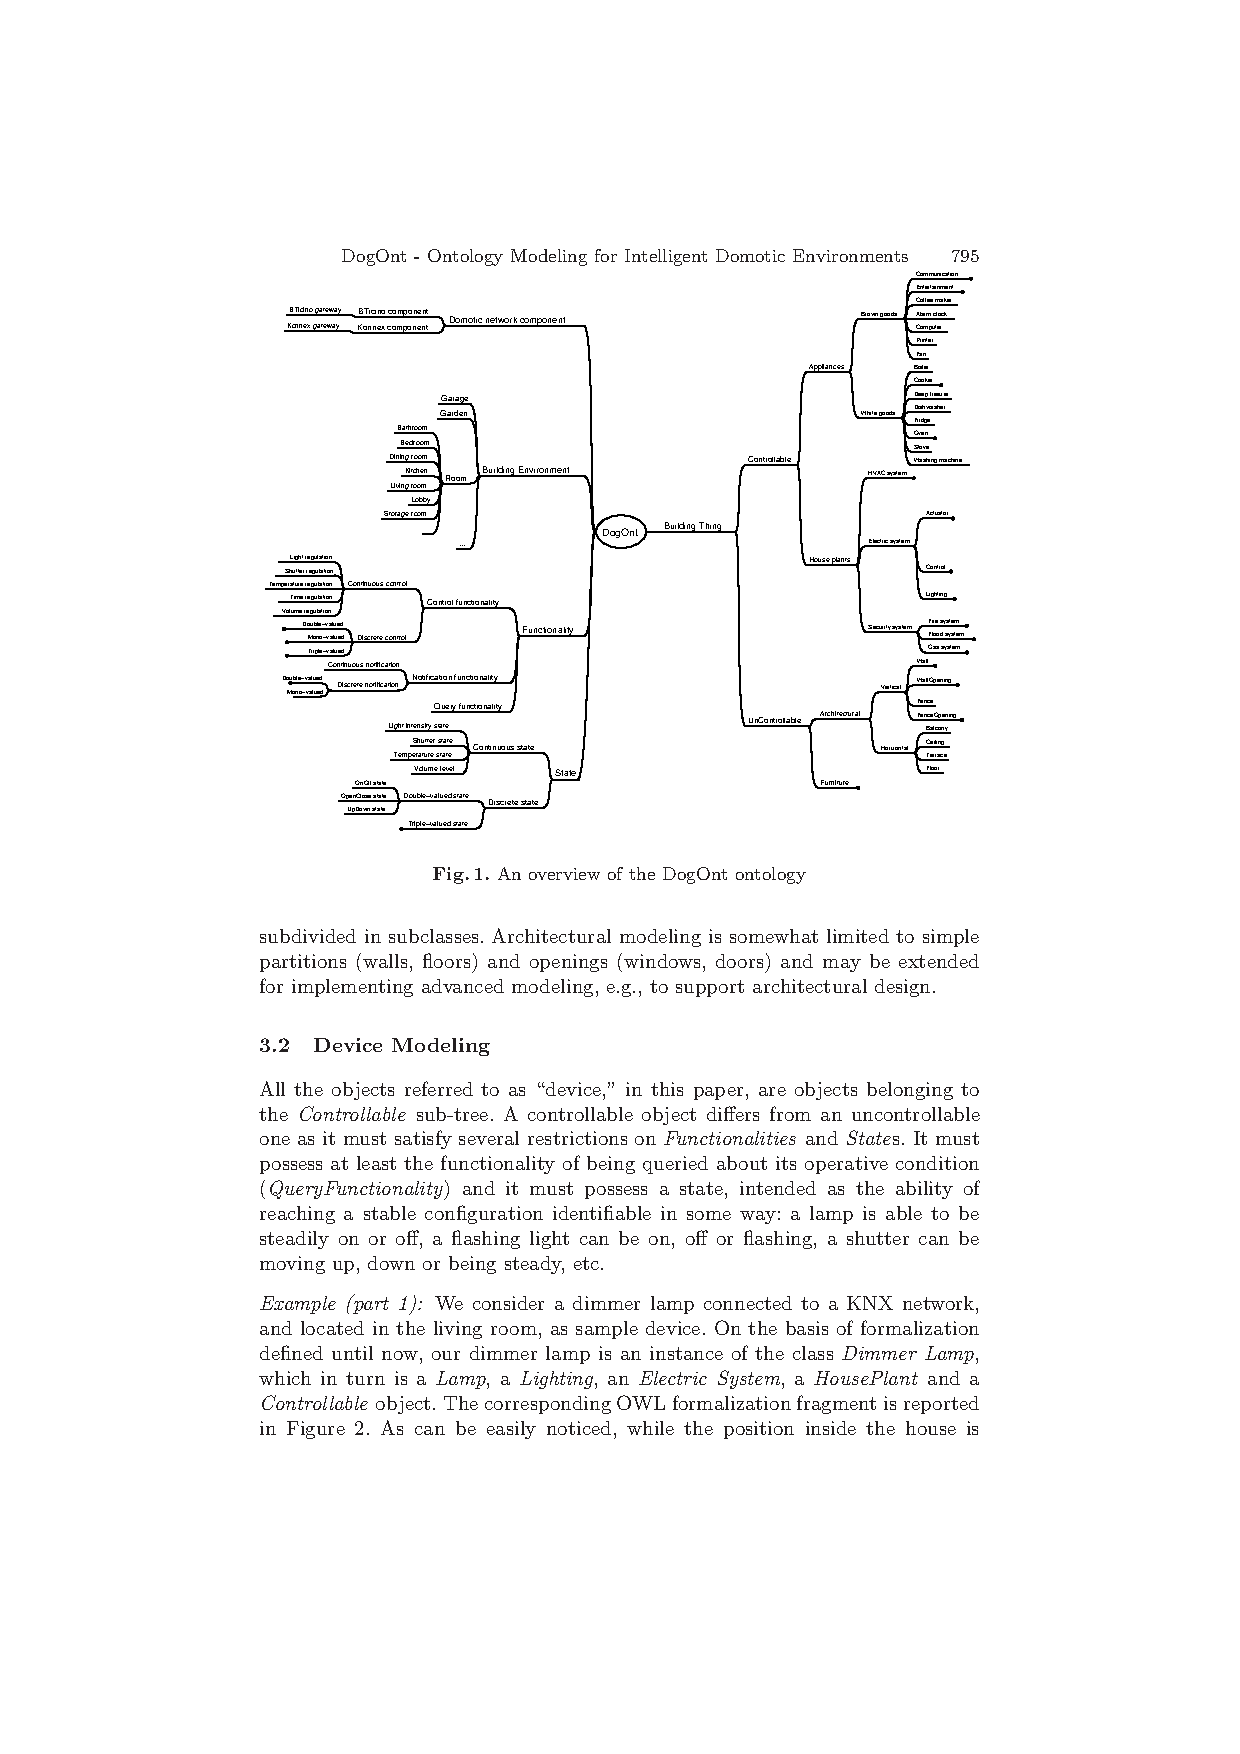
\includegraphics[width=0.8\textwidth, trim=4cm 15.5cm 4cm 4.6cm, clip]{rw-supervision-dogont}
    \caption{L'ontologie de DogOnt}\label{fig:rw:supervision:dogont}
\end{figure}
Pour pouvoir observer, et contrôler, les instances de ces concepts, il est nécessaire de rajouter des fonctionnalités et des variables d'états. Ceci se fait par l'introduction de relations sémantiques telles que \textit{hasControl}, \textit{hasFunctionality}, et \textit{hasState}. En combinant ces associations ainsi que l'ensemble complet des instances, il est possible de représenter l'ensemble des périphériques et leurs capacités.

Plusieurs autres projets ont utilisé ce type de modélisation pour des applications pervasives. Par exemple, Amigo~\cite{BenMokhtar:easy} se focalise plus sur la modélisation des services et des capacités. A contrario, \textit{MATCH}~\cite{Docherty:match} met l'accent sur la hiérarchie des ontologies pour que chaque domaine puisse apporter ses connaissances en utilisant des concepts communs (\textit{dispositifs}, \textit{réseau},\dots).

Nous remarquons que la séparation des domaines permet de gérer les perspectives utilisateurs en fonction de leurs intérêts. De plus, nous notons que l'hétérogénéité des schémas conceptuels est gérée par l'utilisation d'une ontologie commune. La nécessité d'une ontologie commune est récurrente dans ces travaux. Toutefois, dans des travaux récents~\cite{Niang:global,Niang:integration}, il existe des approches semi-automatiques pour intégrer des données de sources hétérogènes via la génération d'une ontologie commune et d'alignements.

\subsubsection{SOCAM : De l'utilité du raisonnement logique}
SOCAM (Service-Oriented Context-Aware Middleware)~\cite{Gu:socam} propose un intergiciel générique pour permettre aux développeurs de créer des applications pervasives par contexte. Cet intergiciel supporte l'acquisition, la découverte, l'interprétation et l'accès aux contextes. Comme les autres solutions présentées jusqu'ici, il s'appuie sur une ontologie conceptualisée comme celle de \textit{MATCH} afin de pouvoir être générique et y apporter les connaissances de chacun des domaines.

L'architecture de SOCAM, représentée en figure~\ref{fig:rw:supervision:socam} qui se décrit en trois 4 composants principaux.
\begin{figure}[ht]
    \centering
    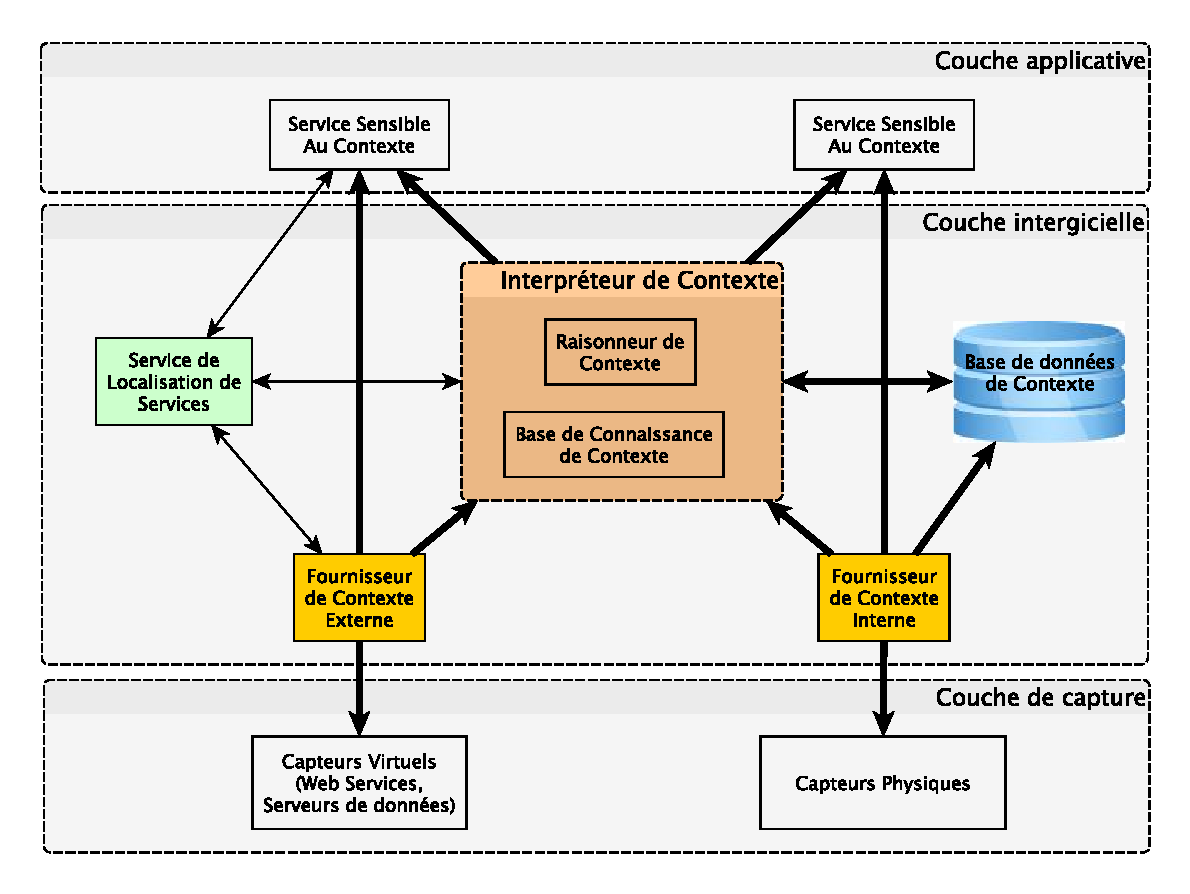
\includegraphics[width=0.66\textwidth]{rw-supervision-socam}
    \caption{Architecture de SOCAM}\label{fig:rw:supervision:socam}
\end{figure}
\begin{itemize}
	\item[\textbf{Fournisseurs de contexte}] Qui permet d'abstraire l'hétérogénéité des données issues des différentes sources (internes, tels que les capteurs ou autres dispositifs), ou externe (services météo ou autres) pour les convertir en \textit{OWL}.
    \item[\textbf{Interpréteur de contexte}] Fournit la logique de raisonnement sur le contexte.
    \item[\textbf{Base de données de contexte}] Stocke les ontologies de contexte et l'historique des contextes pour chaque sous-domaine.
    \item[\textbf{Service de localisation de services}] Sert de catalogue des services externes disponibles. Sa sélection peut se faire sur un type de service, mais il peut aussi faire une comparaison sur le contexte que le service fournit.
\end{itemize}
Les services applicatifs utilisant la notion de contexte vont ainsi utiliser les fonctionnalités que fournit SOCAM pour gérer cet ensemble de données. Une manière classique de construire ces services est de spécifier des actions déclenchées par un ensemble de règles au moment où le contexte change.

SOCAM implémente deux manières de faire de l'inférence logique de prédicats. La première est l'inférence structurelle. En effet, l'application d'une propriété transitive à un concept nous donne plusieurs informations. Par exemple, nous pouvons inférer que l'appareil \textit{Livebox} est une passerelle internet. Or, tous les équipements de cette catégorie ont des propriétés telles que la capabilité à gérer les règles de routage. La deuxième manière d'inférer des informations est un ensemble de règles utilisateurs. En utilisant un moteur similaire aux moteurs \textit{Prolog}, il est possible d'induire des informations qui constituent l'ensemble des situations. Par exemple, les auteurs présentent l'inférence du triplet \textit{(user socam:status 'SLEEPING')} par la détection de la position allongée dans la chambre avec la lumière éteinte.

Nous remarquons ici la présence d'une couche de traitement de données entre les sources et les services qui les utilisent. Cette couche se base sur des inférences logiques qui utilisent un support persistant pour constituer son contexte.

\subsection{Synthèse}
En conclusion, le traitement contextuel des données permet de gérer l'hétérogénéité sémantique des données. Les capacités de traitements sont liées à l'inférence logique pour enrichir la base des connaissances accumulées. Ainsi, il est possible de construire un espace de contexte et d'en inférer des situations de haut niveau. Cette capacité d'abstraction est nécessaire pour l'informatique ubiquitaire qui a besoin de manipuler des concepts humains.

Pour notre problématique d'observation, il reste difficile de gérer l'évolution des données au cours du temps. La liberté d'expression des bases de connaissances fait que l'inférence est complexe à manipuler. Plusieurs travaux s'attellent à permettre aux connaissances et aux règles d'introduire la dimension dynamique~\cite{Weikum:webknowledge, Hellerstein:declarative}. L'apport de cette dimension est toutefois difficile d'un point de vue théorique.

\begin{table}[!ht]
\criteretabDonnee
    {Structure sémantique à base de triplet.}
    {Utilisation d'ontologies. Gestion des contraintes et de l'inférence structurelles variable suivant l'expressivité du langage. En général, \textit{OWL Lite} est utilisé.}
    {Pas de gestion explicite du dynamisme en dehors d'annotations.}
\criteretabTraitement
    {Instantané uniquement.}
    {Les sources s'intègrent en se conformant à un modèle commun. Si tel n'est pas le cas de façon native, des règles d'alignements d'ontologies sont à fournir.}
    {Paradigme déclaratif en général dérivé de programmation logique allant de \textit{Prolog} à \textit{SPARQL}.}
    {Cela part de la logique du premier ordre complète à la capacité de l'algèbre relationnelle (\textit{datalog} non récursif avec négation)}
\criteretabAdaptabilite
    {Nécessité de spécifier des ontologies de domaines pour donner la structure des concepts du système.}
    {La séparation des domaines et le rattachement des données aux domaines permettent de clairement spécifier les différentes perspectives.}
    {Pas d'extensibilité possible sur le traitement d'inférence. Par contre, il est possible suivant l'architecture du système final de créer des capteurs de contextes pour fournir des données logiques de haut niveau.}
    {La complexité de l'inférence peut aller jusqu'en \textit{EXPTIME}. Toutefois, plusieurs implémentations optimisées permettent de traiter des millions de triplets en quelques secondes.}
\caption{Synthèse de l'informatique contextuelle}\label{tab:rw:supervision:contexte:synthese}
\end{table}

\section{Entrepôts de données}
asdwd
\section{Gestion de flux de données}
Devant la multiplication des applications à base de flux de données telles que : la gestion des données de capteurs ou la surveillance réseau, les systèmes de gestions de flux de données (\textit{SGFD}) ont étés conçus. L'idée principale de ce type de système étant de permettre une utilisation des flux de données de la même manière que les bases de données. L'interrogation des flux passerait donc par un langage déclaratif (tout comme le \textit{SQL}) avec un grand pouvoir d'expression.
\subsection{Approche des SGFD}
Un flux de données est une série de données qui s'accumule au fur et à mesure du temps. De façon général, il n'est pas supposé une régularité temporelle sur l'arrivée des données dans le flux (tel que \enquote{\it une donnée toutes les 5 secondes}). L'idée de faire une interrogation sur ces flux de données au sens \enquote{gestion de base de données} du terme n'a pas de sens car il y aurait confusion entre les modes d'interrogations continues et instantanées présentés en section~\ref{sec:rw:supervision:criteres:traitement}. En effet, le paradigme des requêtes est fondamentalement différent~\cite{Gurgen:sstreamware}.
\begin{figure}[ht]
    \centering
    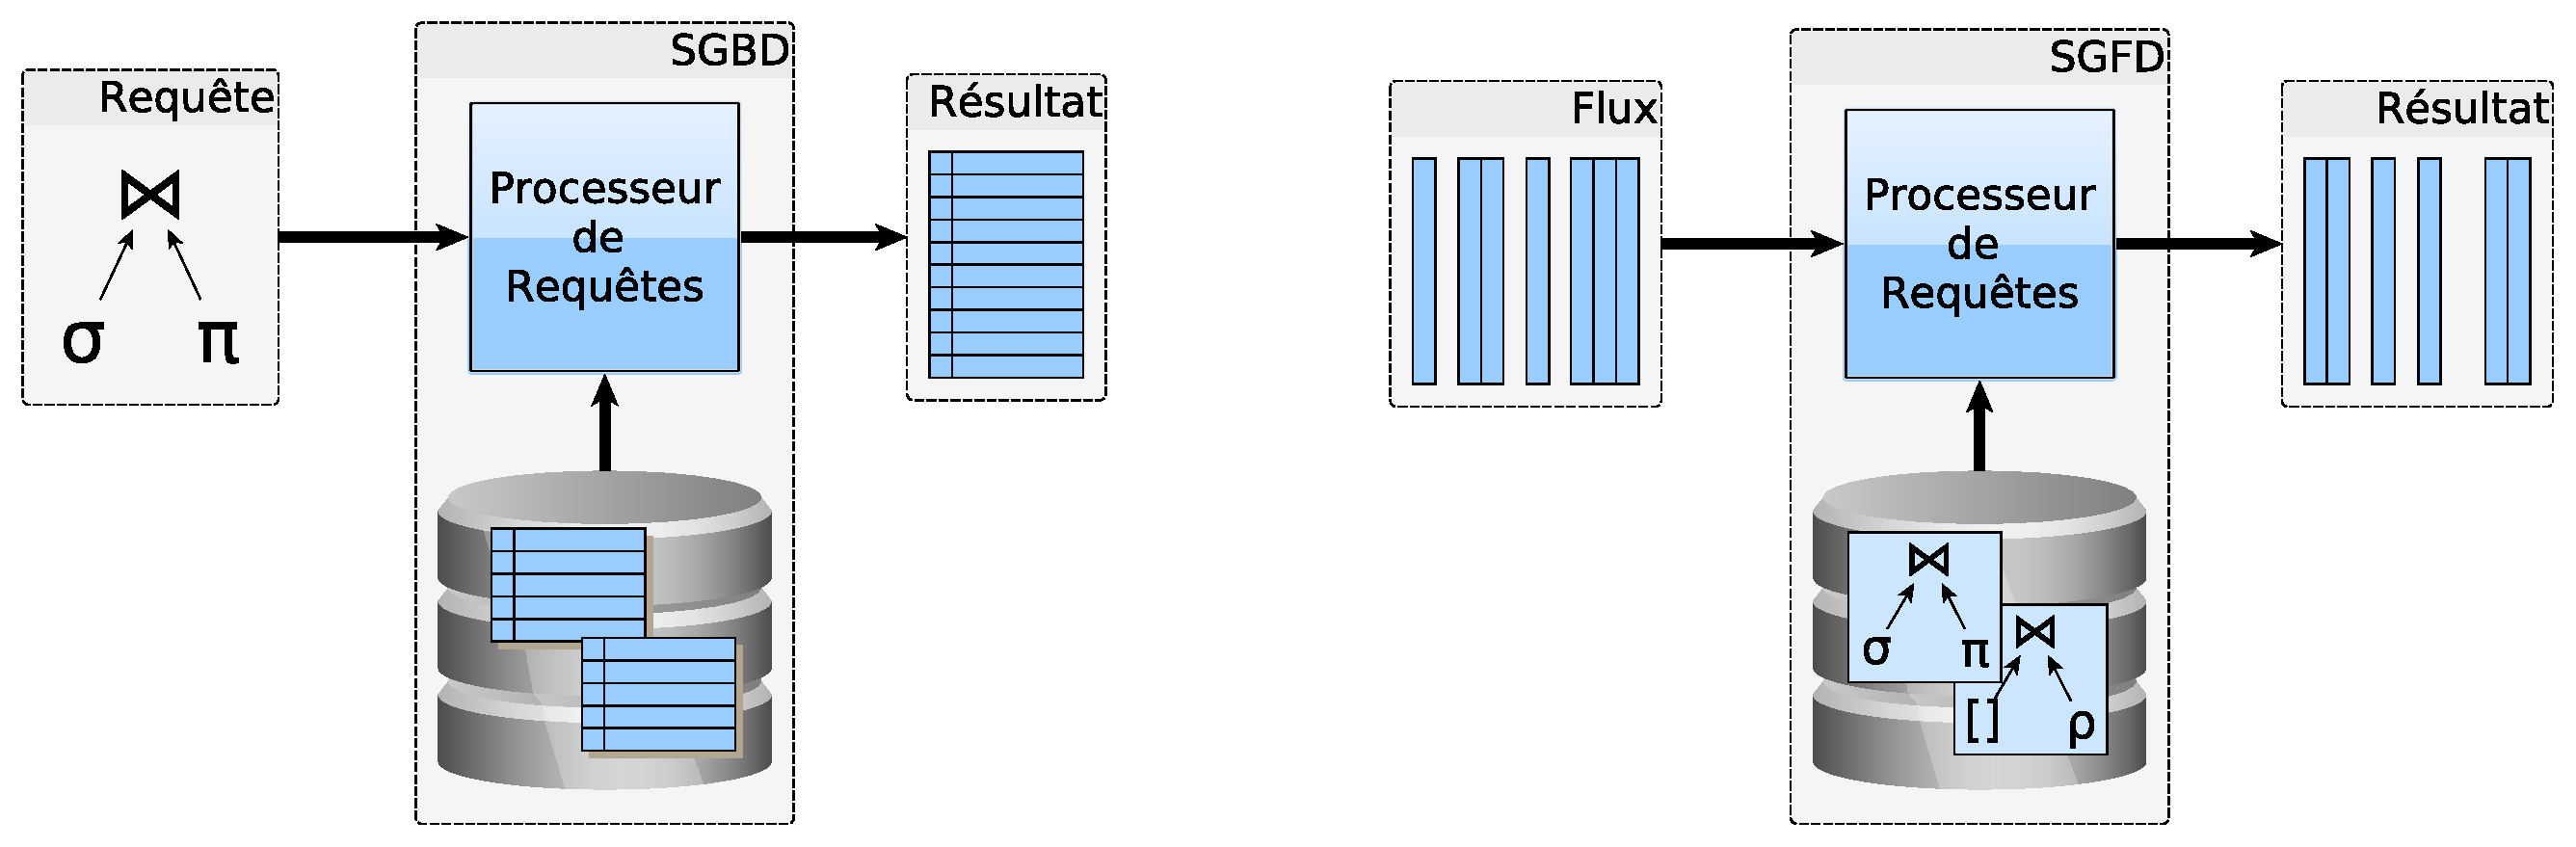
\includegraphics[width=0.75\textwidth]{rw-supervision-sgbd-sgfd}
    \caption{SGBD : Requêtes transitoires, Données persistantes vs SGFD : Données transitoires, Requêtes persistantes}
\end{figure}

\begin{itemize}
    \item[\textbf{Base de données}] : Une requête est une question posée sur un ensemble de relations figées et persistants (principe transactionnel). La réponse est un ensemble de n-uplets. Une fois la requête traitée elle n'existe plus.
    \item[\textbf{Flux de données}] : Une requête un ensemble d'opérateurs et est considéré comme persistant. Le ou les flux de données sont appliqués sur cet ensemble d'opérateurs pour en produire un nouveau flux.
\end{itemize}

\subsection{Principes architecturaux}
\subsection{Les opérateurs}
\subsection{Synthèse}
\begin{table}[!ht]
\criteretabDonnee
    {Modèle dérivé du relationnel mais où le contenu est variable dans le temps.}
    {Pas de structure sémantique en dehors de gestion de méta-données.}
    {Toutes les données sont dynamiques et événementielles a priori.}
\criteretabTraitement
    {Continue.}
    {Il est supposé que chaque source produit un flux de données. Le fait de traiter ces flux participe à l'intégration de sources.}
    {Langages de requêtes similaires aux SQL supportant la dynamique et l'évolution des données}
    {A un instant donné, les opérateurs sont semblables au relationnel. L'expressivité du support du dynamisme reste inconnu encore.}
\criteretabAdaptabilite
    {Création de source pour fournir les flux de données. Comme il n'y a pas de structure sémantique, l'adaptation n'est que l'écriture de requêtes continues.}
    {Pas de perspectives métiers.}
    {Les sources et puits sont en général adaptés par les utilisateurs. Un développement peut être fait dessus, mais il est rarement possible de rajouter des opérateurs.}
    {Très rapide car la latence de traitement doit être contrôlée pour supporter des haut débits.}
\caption{Synthèse des systèmes de gestion de flux de données}\label{tab:rw:supervision:sgfd:synthese}
\end{table}

\section{Conclusion}
Après 20 années de recherche, la gestion de flux de données devient désormais suffisamment mature pour être appliqué massivement. Plusieurs produits commerciaux sont d'ailleurs maintenant utilisés en production. Toutefois, nous pouvons nous rendre compte que la complexité théorique de ces systèmes a été sous-estimé. De nombreux modèles ont été décrit pour représenter les flux de données et leurs traitements. Ces modèles sont encore remis en questions aujourd'hui au fur et à mesure des applications concrètes. 

Nous avons vu que le problème d'avoir une bonne connaissance du modèle et du comportement théorique des SGFD est crucial. En l'état, l'intégration des supports persistants reste ad-hoc et assisté par l'utilisateur. Un fonctionnement intégré avec une modélisation générique capable de gérer les deux modes d'interrogations de façon unifiée est donc indispensable pour manipuler correctement flux et relations persistantes. Similairement, les contributions sur l'optimisation de traitement des requêtes sont encore principalement ponctuelles. Afin d'appliquer un traitement efficace pour toute requête, il est nécessaire d'avoir une bonne connaissance théorique du traitement.

Notre contribution technique se concentrera sur trois points principaux :
\begin{itemize}
 \item[\textbf{Modélisation}] : Création d'Astral, algèbre de traitement des requêtes continues sur flux et relations temporelles. Nous accorderons de l'importance sur la prise en compte des problèmes relevés en section~\ref{sec:rw:sgfd:modeles:synthese}. Cette algèbre sera présenté dans le chapitre~\ref{chap:contrib:astral}
 \item[\textbf{Exécution}] : Mise en œuvre de l'intergiciel Astronef pour construire et exécuter efficacement une requête exprimée avec l'algèbre Astral. Ainsi, à partir d'une requête algébrique, il est possible de sélectionner le plan de requête qui semble le plus efficace grâce aux connaissances accumulés. Cette mise en œuvre sera développée dans le chapitre~\ref{chap:contrib:execution}.
 \item[\textbf{Persistance}] : Conception de l'extension Asteroid permettant l'intégration des requêtes continues sur flux et des requêtes sur support relationnel persistant. Ceci permettra de gérer la représentation du système observé ainsi que l'historisation des données dynamiques. Le support mathématique de cette intégration sera supporté par Astral et sa mise en œuvre par Astronef. Cette intégration sera effectuée dans le chapitre~\ref{chap:contrib:persistance}.
\end{itemize}

Grâce à ces contributions, il deviendra possible de mettre en œuvre un système d'observation générique applicable sur tout type de données. L'utilisateur devra exprimer des requêtes dans le langage algébrique Astral. Une fois ces requêtes écrites, nous serons garanti de leur mise en œuvre. Le tableau~\ref{tab:rw:contrib} résume l'ensemble des points d'analyses que nous nous étions fixés en section~\ref{sec:rw:supervision:criteres}.
\begin{table}[!ht]
\criteretabDonnee
    {Relationnel dérivé. Nous réutilisons les principes utilisés dans la gestion de flux et des bases de données.}
    {\good Modèle entité-relation augmenté pour supporter les flux.}
    {\good Requêtes sur tout type de données (flux, relations).}
\criteretabTraitement
    {\good Continue, Instantannée, Mixte}
    {\good Utilisation des requêtes continues des SGFD en tant qu'intégrateur.}
    {\meh Astral : langage de requête algébrique. Un langage purement déclaratif reste toutefois dérivable de ces fondations théoriques.}
    {\good Relationnel avec support \textbf{intégré} du dynamisme des données.}
\criteretabAdaptabilite
    {\good Spécification du modèle du système ainsi que des requêtes d'intégration (algébriques).}
    {\meh Pour l'analyse, la gestion de données multi-dimensionnelles des entrepôts utilisés est utilisé. Pour l'interrogation continue, utilisation d'un opérateur de préférences sur les flux.}
    {\good Infrastructure générique capable de supporter l'ajout d'opérateurs avec plusieurs implémentations.}
    {\good Héritage de l'efficacité des flux de données. Sélection du meilleur plan d'exécution pour chaque requête. Héritage des supports de grands volumes grâce aux entrepôts.}
\caption{Résumé de notre contribution selon nos critères}\label{tab:rw:contrib}
\end{table}
